\chapter{拉曼效应}
\label{ch:Raman}

当暴露在振荡电磁场中时,介质中的电子由于质量较小,几乎会立即做出反应。而这些电子绕其运行的原子核由于质量相对较大,反应速度要慢得多。因此,影响某一光纤段脉冲特定瞬间的非线性相移取决于两点: 该瞬间脉冲的光功率和过去影响该位置的光功率。材料晶格中原子核的延时机械振动对电磁场的非线性影响被称为 “拉曼效应”~\cite{Raman_original}。 


\section{拉曼响应函数}
在数学上,拉曼效应对光脉冲的影响可以用以下公式描述
\begin{align}
\label{eq:raman}
 \partial_z \A = i\gamma\left( 
\A \int_{0}^{\infty} R(T_{delay})|\A(z,T-T_{delay})|^2 dT_{delay} \right),
\end{align}
在忽略损耗、色散和自陡的情况下,它等价于公式 ~\ref{eq:GNLSE}。函数 $R(T_{delay})$ 是总响应函数,表示过去不同时间的功率对给定瞬间影响脉冲的非线性相移的贡献程度。它可以通过三角函数写成电子响应的瞬时贡献与晶格振动引起的延迟拉曼响应之和,即
\begin{align}
    \label{eq:response}
    R(T_{delay})&= (1-f_R)\delta(T_{delay})+f_Rh_R(T_{delay}),
\end{align}
其中,$0\leq f_R\leq 1$ 是一个标量,决定了两个贡献的相对大小。拉曼响应函数的确切函数形式 $h_R(T_{delay})$ 取决于材料,但通常类似于一个乘以阻尼项的正弦函数,并且必须满足 $\int_{-\infty}^{\infty}h_R(T_{delay}) dT_{delay}=1$,因为它本质上是 “权衡 ”过去不同时间的功率对当前非线性相移的贡献程度。 此外,必须要求 $h_R(T_{delay})=0$ for $T_{delay}\leq0$ 以防止该表达式违反因果关系,让 \emph{future} 功率影响当前的非线性相移。请参阅 \href{https://www.desmos.com/calculator/bdg6icprch}{此交互图},了解过去的功率对拉曼效应引起的相移的影响。
直观地说,函数 $h_R(T_{delay})$就像描述音叉、钢琴键或吉他弦突然被敲击后声波振幅的函数一样,是一种逐渐 “回落 ”的振荡。继续类比,如果把 $|\A(z,T-T_{delay})|^2$ 看作是在不同时间具有不同强度的瞬时击打的大集合,那么当前的振荡取决于过去的所有振荡就说得通了。 
将公式 ~\ref{eq:response}代入公式 ~\ref{eq:raman},并对三角函数进行积分求得
\begin{align}
    \label{eq:raman_split}
    \partial_z \A = i\gamma\A\left( 
(1-f_R)|\A(z,T)|^2+f_R \int_{0}^{\infty} h_R(T_{delay})|\A(z,T-T_{delay})|^2 dT_{delay} \right).
\end{align}
请注意,如果脉冲功率的变化与响应函数的持续时间相比非常缓慢,则可以近似地计算 $h_R(T_{delay})\approx \delta(T_{delay})$(或者,等价地计算 $|\A(z,T-T_{delay})|^2\approx|\A(z,T)|^2$),在这种情况下,公式~\ref{eq:SPM}就恢复了。换句话说,只有当脉冲持续时间接近分子晶格自然振荡的持续时间时,拉曼效应才会明显!假设脉冲持续时间明显长于 $h_R(T_{delay})$的持续时间,因此不同时间延迟下的功率可以通过将当前功率及其梯度线性外推到过去来找到,那么公式~\ref{eq:raman_split}中的积分可以写为 
\begin{align}
\label{eq:raman_approx}
    f_R \int_{0}^{\infty} h_R(T_{delay})|\A(z,T-T_{delay})|^2 dT_{delay} &\approx\\ \nonumber \quad\quad\quad f_R \int_{0}^{\infty} h_R(T_{delay})\left[ 
  |\A(z,T)|^2-T_{delay}\partial_T|\A(z,T)|^2 \right] dT_{delay} &=\\ \nonumber \quad\quad\quad  |\A(z,T)|^2f_R- \partial_T|\A(z,T)|^2 f_R\int_{0}^{\infty} T_{delay} h_R(T_{delay}) 
   dT_{delay}&=\\ \nonumber \quad\quad\quad  |\A(z,T)|^2f_R- \partial_T|\A(z,T)|^2 T_R &,
\end{align}
其中 $T_R$ 是拉曼响应函数的平均持续时间,用 $f_R$ 缩放。将公式~\ref{eq:raman_approx}的结果代入公式~\ref{eq:raman_split}可得
\begin{align}
    \label{eq:raman_approx_applied}
\partial_z \A = i\gamma\A\left( 
|\A(z,T)|^2-T_R \partial_T|\A(z,T)|^2\right),
\end{align}
其中包含与电流功率成比例的 “常规 ”SPM 项,以及取决于功率时间导数的附加项。对于二氧化硅,$T_R/approx 3$~fs,因此公式 ~\ref{eq:raman_approx_applied}将对超过约 600~fs 的脉冲有效。公式 ~\ref{eq:raman_approx}中应用的近似值可以扩展到包括 $|\A(z,T)|^2$ 的二阶导数,以提高精确度。从公式 ~\ref{eq:SPM_example} 和 Fig.~\ref{fig:chirp_profiles} 中回想一下,“常数 ”SPM 项会导致瞬时频率大幅下降,而此时功率的 \emph{derivative} 值非常正(原文如此)。根据同样的逻辑,公式 ~\ref{eq:raman_approx_applied}中的拉曼项会导致 “导数的导数 ”为负的瞬时频率大幅下降。换句话说,拉曼效应会在脉冲峰值处产生红移,而在其他地方不会产生等效的大蓝移,从而使整个脉冲 “更红”!从物理学角度来看,红移的产生是因为入射光子会激发介质晶格的机械振动,从而损失部分能量。
\subsection{$h_R(T_{delay})$的表达式}
假设分子振动以单一频率为主,二氧化硅中拉曼效应的近似表达式为 
\begin{align}
\label{eq:raman_basic}
    h_R^{basic}(T_{delay})&= \left(\frac{1}{\tau_1^{2}}+\frac{1}{\tau_2^{2}} \right)\tau_1\exp\left(-\frac{T_{delay}}{\tau_2}\right)\sin\left(\frac{T_{delay}}{\tau_1}\right),
\end{align}
其中 $f_R=0.18$,$\tau_1=12.2$~fs,$\tau_2=32$~fs。为了尊重因果关系,所有列出的 $h_R(T_{delay})$表达式都假定 $T_{delay}\leq0$ 为零。在数学上,这可以通过乘以 Heaviside 阶跃函数来确保。对于二氧化硅的振动行为,比公式 ~\ref{eq:raman_basic} 更精确的近似值是  
\begin{align}
\label{eq:raman_new}
    h_R^{better}(T_{delay})&= (1-f_b) h_R^{basic}(T_{delay})+f_b\frac{2\tau_b-T_{delay}}{\tau_b^2}\exp\left(-\frac{T_{delay}}{\tau_b}\right),
\end{align}
其中,$f_R=0.245$,$f_b=0.21$,$\tau_b=96$~fs。二氧化硅拉曼响应的精确表达式为
\begin{align}
\label{eq:Raman_exact}
    h_R^{exact}(T_{delay})&=c^{-1}_{norm}\sum_{n=0}^{12}C_n\exp\left(- g_nT_{delay}-0.25G_n^2T^2_{delay}  \right)\sin\left(2\pi \nu_nT_{delay} \right),
\end{align}
其中,$f_R=0.18$,参数$C_n$、$g_n$、$G_n$和$\nu_n$列于表 ~\ref{tab:raman_coeffs},$c_{norm}=3.75225$~ps,因此$\int_0^\infty h_R^{exact}(T_{delay}) dT_{delay}=1$。图 ~\ref{fig:raman_combined}展示了这三种二氧化硅拉曼响应模型的可视化及其对同一光脉冲的影响。图 ~\ref{fig:raman_combined}~b) 中绘制了 $h_R(T_{delay})$ 不同表达式的傅立叶变换虚部。从物理角度看,这些光谱意味着拉曼效应允许特定光学频率从其上方 13~THz 的频率 “窃取 ”功率,并迫使其向下方 13~THz 的频率 “捐赠 ”功率。由于与章节 ~\ref{sec:KK_relations}中所述的原因类似,光谱的实部(未显示)与拉曼效应引起的折射率变化有关,因此可以确定其引起的时间延迟。根据图 ~\ref{fig:raman_combined}~b) 中所示曲线的最大值,最大拉曼增益以及拉曼效应变得显著的特征长度可以表示为
\begin{align}
    g_{Raman} &= \frac{4}{3} \gamma f_R P_0 n(\omega_0)\cdot \text{max}( \text{Im} \{ \FT \{ h_R(T_{delay}) \}(\omega) \} )\\ 
    L_{Raman} &= \frac{1}{g_{Raman}},
\end{align}
其中,$P_0$ 是脉冲的最大功率,$n(\omega_0)$ 是介质的折射率(对于二氧化硅,折射率约为 $1.47$)。有关拉曼效应的更多信息,请参见 \href{https://www.youtube.com/playlist?list=PLdFybGSAoPnn6tnSmptR71zKAgcKsjIfi}{这些视频教程}。  
\begin{table}
\begin{center}
    \begin{tabular}{c|c|c|c|c}
    \label{tab:raman_coeffs}
        n  &$C_n$ & $g_n$ [fs] & $G_n$ [fs] & $\nu_n$ [THz]  \\ \hline
        0  &  1    &0.521       &1.562          &1.69   \\
        1  &  11.4 &1.163       &3.310          &3.00   \\
        2  &  36.67&1.749       &5.246          &6.93   \\
        3  &  67.67&1.624       &4.872          &10.87\\
        4  &  74   &1.352       &4.057          &13.88       \\
        5  &  4.5  &0.245       &0.734          & 14.90   \\
        6  &  6.8  &0.415       &1.244          & 18.33   \\
        7  &  4.6  &1.549       &4.647          & 20.74   \\
        8  &  4.2  &0.594       &1.784          & 23.79  \\
        9  &  4.5  &0.642       &1.928          & 25.05   \\
        10 &  2.7  &1.499       &4.497          & 27.88   \\
        11 &  3.1  &0.909       &2.728          & 32.38   \\
        12 &  3    &1.599       &4.797          &   36.42 
    \end{tabular}
    \caption{公式~\ref{eq:Raman_exact}中二氧化硅拉曼响应精确表达式的参数表,由 \cite{raman_exact}修改而来。  }
    \end{center}
\end{table}

\begin{figure}
    \centering
    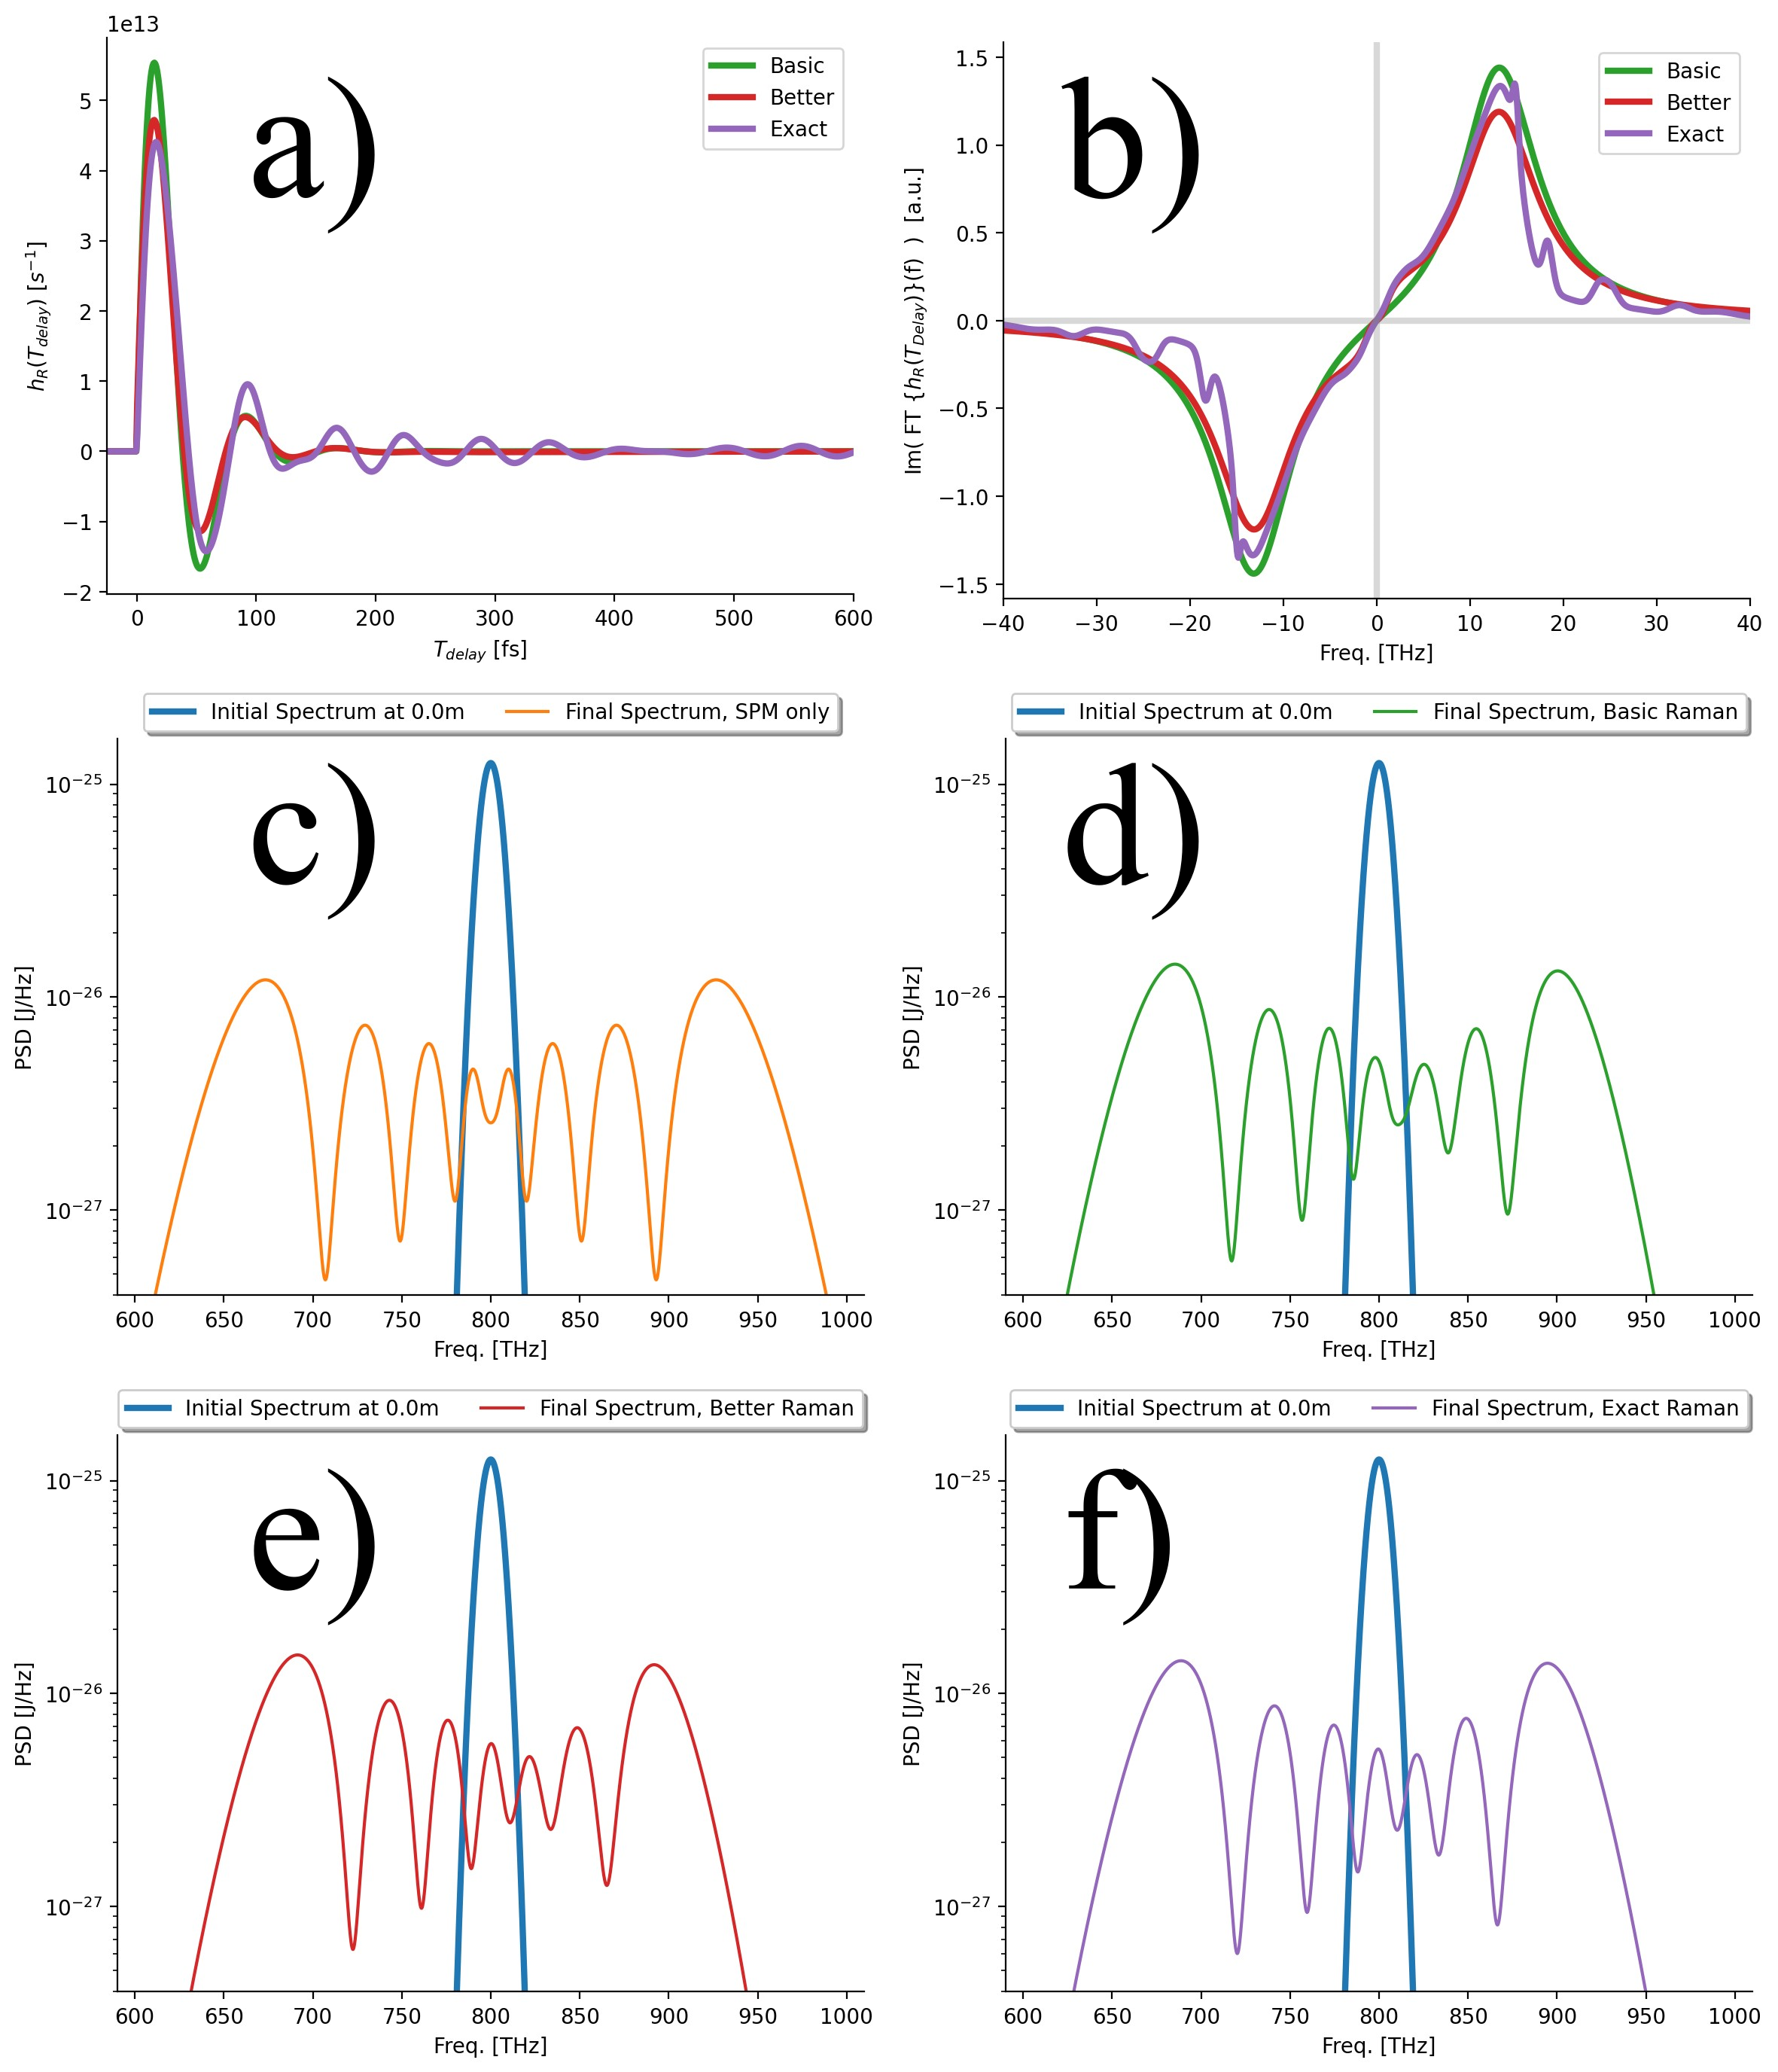
\includegraphics[width=1\linewidth]{figures/Raman_combined.png}
    \caption{a) Eq.~\ref{eq:raman_basic}(绿色)、Eq.~\ref{eq:raman_new}(红色)和 Eq.~\ref{eq:Raman_exact}(紫色)的时域图。) c) 仅受 SPM 影响的脉冲的初始和最终光谱。 d) 受公式 ~\ref{eq:raman_basic} 描述的拉曼效应影响的与 c) 中相同脉冲的初始和最终光谱。e) 与 d) 相同,但 Eq.~\ref{eq:raman_new} f) 与 d) 相同,但 Eq.~\ref{eq:Raman_exact}. 这些图是使用 \href{https://colab.research.google.com/drive/1TqixCGQ51DVwpB3VA6J1XQCpDcf4xwb4?usp=sharing}{这个交互式笔记本}生成的,鼓励读者尝试使用。}
    \label{fig:raman_combined}
\end{figure}




